%%
%% This is file `sample-sigconf.tex',
%% generated with the docstrip utility.
%%
%% The original source files were:
%%
%% samples.dtx  (with options: `sigconf')
%% 
%% IMPORTANT NOTICE:
%% 
%% For the copyright see the source file.
%% 
%% Any modified versions of this file must be renamed
%% with new filenames distinct from sample-sigconf.tex.
%% 
%% For distribution of the original source see the terms
%% for copying and modification in the file samples.dtx.
%% 
%% This generated file may be distributed as long as the
%% original source files, as listed above, are part of the
%% same distribution. (The sources need not necessarily be
%% in the same archive or directory.)
%%
%%
%% Commands for TeXCount
%TC:macro \cite [option:text,text]
%TC:macro \citep [option:text,text]
%TC:macro \citet [option:text,text]
%TC:envir table 0 1
%TC:envir table* 0 1
%TC:envir tabular [ignore] word
%TC:envir displaymath 0 word
%TC:envir math 0 word
%TC:envir comment 0 0
%%
%%
%% The first command in your LaTeX source must be the \documentclass command.
\documentclass[sigconf]{acmart}

%%
%% \BibTeX command to typeset BibTeX logo in the docs
\AtBeginDocument{%
  \providecommand\BibTeX{{%
    \normalfont B\kern-0.5em{\scshape i\kern-0.25em b}\kern-0.8em\TeX}}}

%% Rights management information.  This information is sent to you
%% when you complete the rights form.  These commands have SAMPLE
%% values in them; it is your responsibility as an author to replace
%% the commands and values with those provided to you when you
%% complete the rights form.
% \setcopyright{acmcopyright}
% \copyrightyear{2018}
% \acmYear{2018}
% \acmDOI{XXXXXXX.XXXXXXX}

%% These commands are for a PROCEEDINGS abstract or paper.
% \acmConference[Conference acronym 'XX]{Make sure to enter the correct
%   conference title from your rights confirmation emai}{June 03--05,
%   2018}{Woodstock, NY}
% \acmPrice{15.00}
% \acmISBN{978-1-4503-XXXX-X/18/06}


%%
%% Submission ID.
%% Use this when submitting an article to a sponsored event. You'll
%% receive a unique submission ID from the organizers
%% of the event, and this ID should be used as the parameter to this command.
%%\acmSubmissionID{123-A56-BU3}

%%
%% The majority of ACM publications use numbered citations and
%% references.  The command \citestyle{authoryear} switches to the
%% "author year" style.
%%
%% If you are preparing content for an event
%% sponsored by ACM SIGGRAPH, you must use the "author year" style of
%% citations and references.
%% Uncommenting
%% the next command will enable that style.
%%\citestyle{acmauthoryear}

%%
%% end of the preamble, start of the body of the document source.
\begin{document}

%%
%% The "title" command has an optional parameter,
%% allowing the author to define a "short title" to be used in page headers.
\title{Natural Language Processing (NLP) with Disaster tweets}

%%
%% The "author" command and its associated commands are used to define
%% the authors and their affiliations.
%% Of note is the shared affiliation of the first two authors, and the
%% "authornote" and "authornotemark" commands
%% used to denote shared contribution to the research.


\author{Sina Abbasi}
\affiliation{%
  \institution{University of Saskatchewan}
%   \city{Canad}
  \country{Canada}}
\email{sia942@usask.ca}

%%
%% By default, the full list of authors will be used in the page
%% headers. Often, this list is too long, and will overlap
%% other information printed in the page headers. This command allows
%% the author to define a more concise list
%% of authors' names for this purpose.
% \renewcommand{\shortauthors}{Trovato and Tobin, et al.}

%%
%% The abstract is a short summary of the work to be presented in the
%% article.
\begin{abstract}


Twitter is one of the most popular social media these days, and the best place to get breaking news instantly. Monitoring Twitter is interesting for a lot of companies, e.g. disaster relief organizations. In this regard, we are going to build a model for the disaster tweets classification task of whether the tweets are pointing to a real disaster or not. To overcome this problem, we proposed a model using contextualized BERT embedding layer. Our proposed model shows performance improvement in comparison to the base model with LSTM structure in terms of F1 score. The source code can be found here: \url{https://git.cs.usask.ca/sia942/disastertweetsclassification}

\end{abstract}

%%
%% The code below is generated by the tool at http://dl.acm.org/ccs.cfm.
%% Please copy and paste the code instead of the example below.
%%
% \begin{CCSXML}
% <ccs2012>
%  <concept>
%   <concept_id>10010520.10010553.10010562</concept_id>
%   <concept_desc>Computer systems organization~Embedded systems</concept_desc>
%   <concept_significance>500</concept_significance>
%  </concept>
%  <concept>
%   <concept_id>10010520.10010575.10010755</concept_id>
%   <concept_desc>Computer systems organization~Redundancy</concept_desc>
%   <concept_significance>300</concept_significance>
%  </concept>
%  <concept>
%   <concept_id>10010520.10010553.10010554</concept_id>
%   <concept_desc>Computer systems organization~Robotics</concept_desc>
%   <concept_significance>100</concept_significance>
%  </concept>
%  <concept>
%   <concept_id>10003033.10003083.10003095</concept_id>
%   <concept_desc>Networks~Network reliability</concept_desc>
%   <concept_significance>100</concept_significance>
%  </concept>
% </ccs2012>
% \end{CCSXML}

% \ccsdesc[500]{Computer systems organization~Embedded systems}
% \ccsdesc[300]{Computer systems organization~Redundancy}
% \ccsdesc{Computer systems organization~Robotics}
% \ccsdesc[100]{Networks~Network reliability}

%%
%% Keywords. The author(s) should pick words that accurately describe
%% the work being presented. Separate the keywords with commas.
\keywords{Natural Language Processing, BERT, text classification}

%% A "teaser" image appears between the author and affiliation
%% information and the body of the document, and typically spans the
%% page.
% \begin{teaserfigure}
%   \includegraphics[width=\textwidth]{sampleteaser}
%   \caption{Seattle Mariners at Spring Training, 2010.}
%   \Description{Enjoying the baseball game from the third-base
%   seats. Ichiro Suzuki preparing to bat.}
%   \label{fig:teaser}
% \end{teaserfigure}

%%
%% This command processes the author and affiliation and title
%% information and builds the first part of the formatted document.
\maketitle

\section{Introduction}
Nowadays, thanks to smartphones and easy access to the internet across the world, free social media applications are one of the best places to get breaking news instantly. Especially after COVID-19 hit, news consumption from social media rapidly increased, where based on a Pew Research Center survey conducted 31 August - 7 September 2020, about half of US adults (53\%) get their news” often” or” sometimes” from social media; for example, about half of Twitter’s users get their news from there as you can see in Fig. \ref{fig:twitter}. \cite{shearer2021news}. Moreover, people use Twitter to report emergency news that they see in real-time. Therefore, many companies and news agencies are interested in monitoring Twitter to get real-time and breaking news. Besides, organizations such as disaster relief organizations want to know the news about disasters as soon as possible. This monitoring cannot be done by humans because we are dealing with on average 6000 \cite{numTweet} tweets per second. 

\begin{figure}[h]
  \centering
  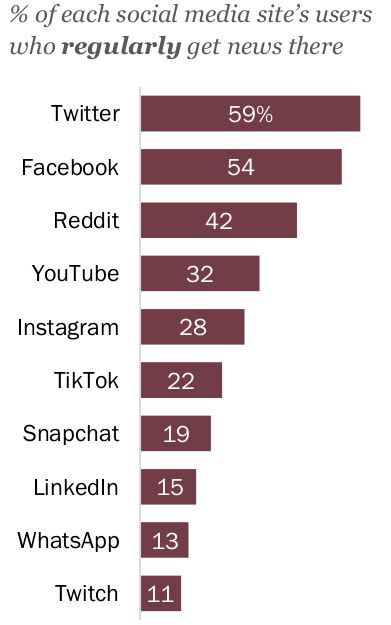
\includegraphics[scale=0.35]{twitter.png}
  \caption{Large portion of Twitter users regularly get news on the site \cite{shearer2021news}.}
  \label{fig:twitter}
\end{figure}

Dataset and task in this project are taken from the Kaggle competition “Natural Language Processing with disaster tweets” \cite{kagglecomp}. The dataset contains 10000 tweets from Twitter that have been extracted by some keywords, e.g., ablaze, accident, death, bleeding, etc. Dataset is human-labeled in the way that which tweets explain a real disaster or not. Subsequently, the task for this project is defined to be classifying tweets based on real and non-real disaster tweets. Pragmatically monitoring tweets by only analyzing the words in each sentence separately is not a promising approach. For example, the author of a tweet said: "On plus side LOOK AT THE SKY LAST NIGHT IT WAS ABLAZE" \cite{tw}; the word "ABLAZE" is used not in actual meaning but metaphorically.

\subsection{related work}
Authors in \cite{sit2019identifying} work on similar datasets but the tweets related to hurricanes. They get the data from Twitter and aim to first classify and then analyze disaster-related tweets. In their binary classification phase, classification methods: LSTM, CNN, SVM, Logistic Regression, and Ridge are performed, and based on their evaluation Long Short-Term Memory (LSTM) gets a better fit to the sequential order of textual data. Looking through the top solutions on the Kaggle website where they used LSTM structure to solve this task, we found and ran a notebook \cite{lstmsol}, which gave us a 0.78 F1 score. This is a decent score for an NLP task. However, based on a new method published by google researchers in 2018 called "BERT: Pre-training of Deep Bidirectional Transformers for Language Understanding". The BERT can learn better contextual text \cite{devlin2018bert}. Therefore, we are going to use this transformer for our task and try to get better F1 performance than LSTM and provide a comparison between them. 

\subsection{contribution}
In this project, we propose a sequential model structure for this binary classification task based on the analysis we did on the dataset. In our proposed model the BERT layer is used as a trainable embedding layer. In addition, based on the discussion in the related works section, we also provide a competitive base model that has an LSTM structure. Our proposed model outperforms the base model in terms of F1 score by a five percent difference. 




\section{Methods}

\subsection{Dataset}

Each sample in the dataset has four columns: 
\begin{itemize}
  \item \textit{id}: a unique identifier for each tweet 
  \item \textit{text}: the text of the tweet
  \item \textit{location}: the location the tweet was sent from
  \item \textit{keyword}: a particular keyword from the tweet
  \item \textit{target} (label): in train data only, this denotes whether a tweet is about a real disaster (1) or not (0). 
\end{itemize}

Fig. \ref{fig:sample} shows five samples of data set. The type of dataset for columns \textit{keyword}, \textit{location}, and \textit{text} columns are String, and the target (label) column is float64. 
\begin{figure}[h]
  \centering
  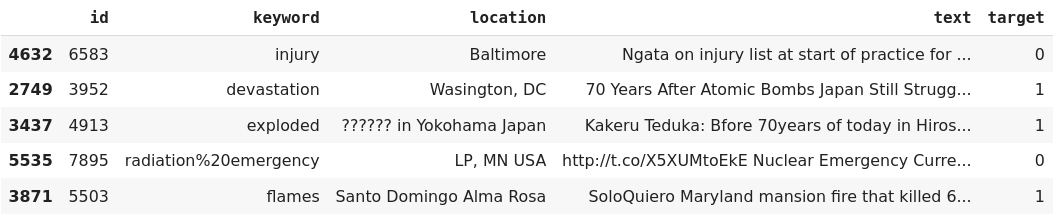
\includegraphics[width=\linewidth]{trainsample.png}
  \caption{Data samples}
  \label{fig:sample}
\end{figure}

Train data contains 7613 samples, and test data has 3263 unlabeled samples. The closest dataset to our dataset was used in \cite{sit2019identifying}. Authors manually labeled 20,000 tweets keyword-based and geo-located corpus of tweets generated before, during, and after Hurricane Irma in its impact area. The dataset has the same features as our dataset, but this dataset is labeled based on only the Hurricane Irma disaster. However, our dataset is more generally related to various kinds of disasters. 

\subsubsection{Dataset set analysis}

Fig \ref{fig:targetdist} depict the label distribution, about 57\% of the data belongs to a non-disaster-tweet class (0) and the rest belong to a disaster-tweet class (1). Therefore, we do not expect class imbalances. A simple inspection showed there are no null values in labels. 
\begin{figure}[h]
  \centering
  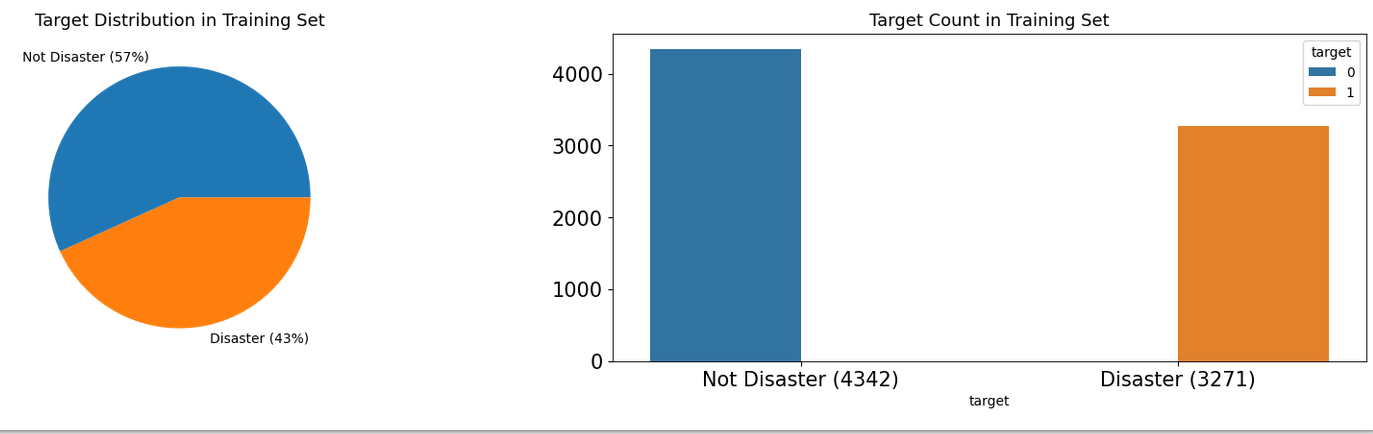
\includegraphics[width=\linewidth]{targetDist.png}
  \caption{Target distribution in training set}
  \label{fig:targetdist}
\end{figure}

We analyzed each input data features separately. The first feature of data is location. this column has lots of Null values and we replaced them with the value unknown. Fig. \ref{fig:locdist} shows the top 10 most frequently locations where the tweet was sent from. As it is clear, lots of data samples have \textit{unknown} locations. Then using this feature does not help the model to get better results and it causes the model to mislead. 
\begin{figure}[h]
  \centering
  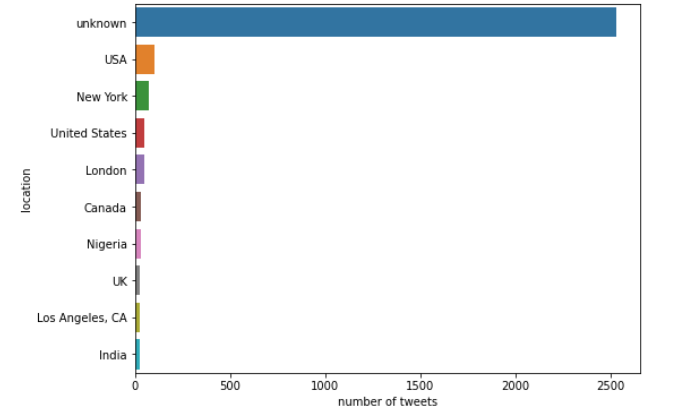
\includegraphics[width=\linewidth]{loc.png}
  \caption{Location distribution in training set}
  \label{fig:locdist}
\end{figure}



The second feature will be the \textit{keyword} feature. In contrast to what we had in the location column; the \textit{keyword} column has some clues. The Fig. \ref{fig:keyword} shows the relation between \textit{keyword}s and \textit{label}s. For example, the words: “debris”, “derailment”, and “wreckage” have been seen in only tweets that relate to a real-disaster class (1). Also, a word like “aftershock” is just used in tweets that point to a non-disaster class (0). In Fig. \ref{fig:keyword}, \textit{keyword}s are sorted by average over labels for each \textit{keyword}, which means that the leftmost word on the x-axis has an average of one (all \textit{label}s corresponding to that \textit{keyword} are equal to one and relate to a disaster). The \textit{keyword} column has 61 null values over all train samples, which we can simply remove those samples from training data.
\begin{figure*}[h]
  \centering
  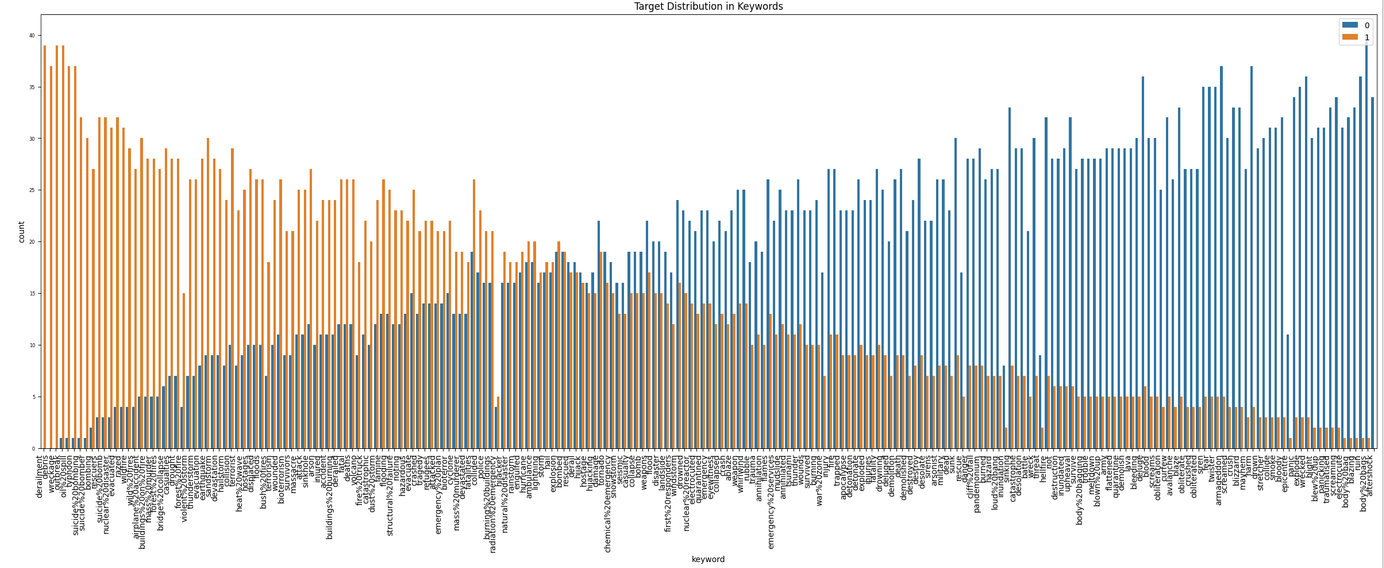
\includegraphics[width=\linewidth]{keyword.png}
  \caption{Target Distribution in Keywords}
  \label{fig:keyword}
\end{figure*}

Finally, we did explore the \textit{text} feature. The most challenging part of this task is cleaning the text column, where we deal with lots of stop words, numbers, dates, punctuation, accent characters, tags, web-links, etc. The preprocessing text has been done not only by removing all tags, web-links, punctuation, stop words, accents, and unknown ASCII characters, but also by converting abbreviated words. Word cloud for each class has been shown in Fig. \ref{fig:wordcloud}.
\begin{figure}[h]
  \centering
  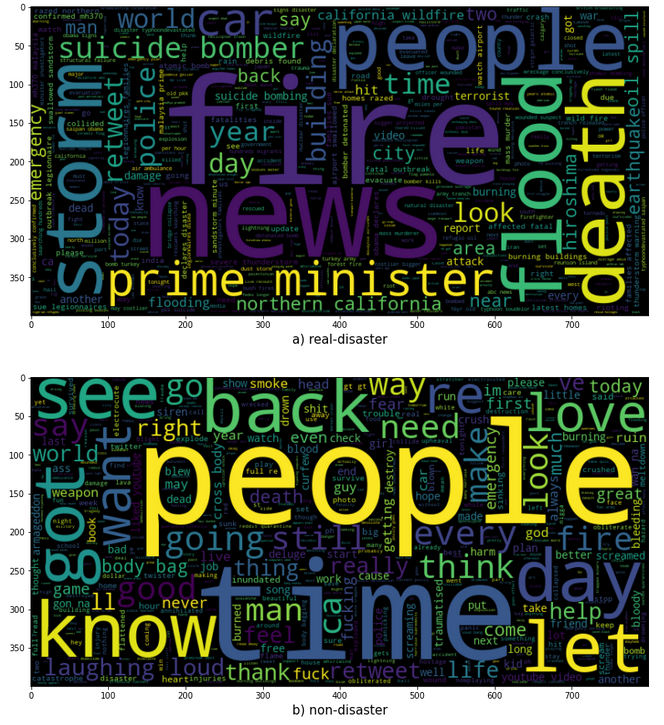
\includegraphics[width=\linewidth]{wordcloud.png}
  \caption{Word cloud after preprocessing \textit{text} feature.}
  \label{fig:wordcloud}
\end{figure}

Based on \ref{fig:wordcloud}, somehow, we can get the sense that which one is related to which classes, and that is why other base model solutions that use simple embedding layers and deep neural networks can get a satisfactory performance. However, in this task, we are aiming one step further to use the BERT transformer that can capture the context relation between words in \textit{text} input to get promising results.

\subsection{Models}
In this section, first we delve into our proposed solution and then we explain our base model. 
\subsubsection{Proposed Model}
We use the BERT transformer and update its parameter through the training process. There are couples of choices for the BERT transformer that we choose to work with the simple one that corresponds to uncased English words and its generated classification token ([‘CLS’]) has 768 entries for each data sample. The classification token generated from BERT is fed to a dense layer with 1024 units, and then the last layer has one unit for classification. Fig. \ref{fig:model} illustrates the structure of proposed model. 
\begin{figure}[h]
  \centering
  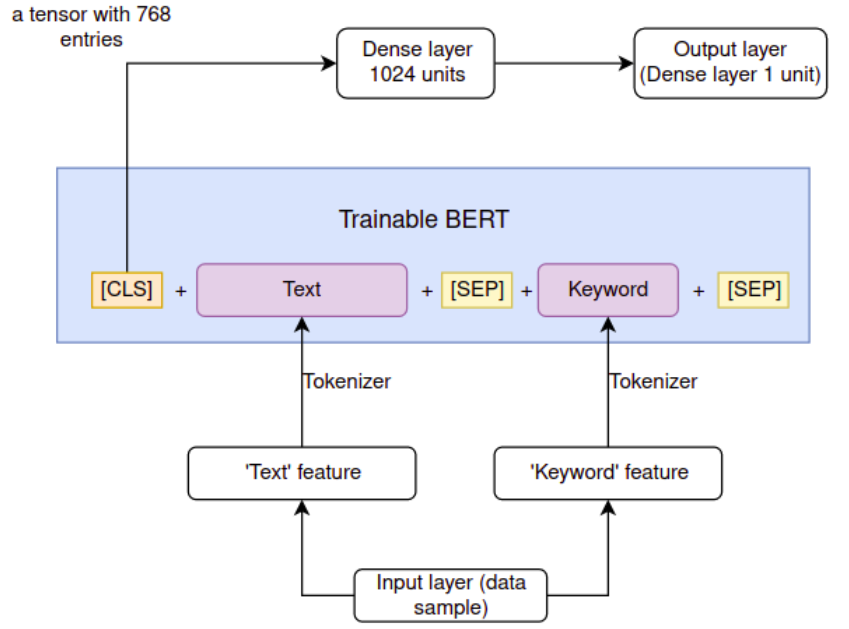
\includegraphics[width=\linewidth]{model.png}
  \caption{Proposed model structure.}
  \label{fig:model}
\end{figure}
Given the analysis in Dataset section, the features that are going to be used are the \textit{text} (text input), and \textit{keyword} column (categorical input) of each data sample. In \cite{gu2021package}, authors executed some experiments on BERT transformer with the dataset that includes various categorical and numerical features along with \textit{text} feature. The authors experimentally proved that categorical features can be added to \textit{text} feature as a new sentence to get a better performance. Therefore, as you can see in Fig. \ref{fig:model}, we added our \textit{keyword} feature to the \textit{text} as second sentence (in BERT model [SEP] token is used to separate the sentences). 

\subsubsection{Base Model}
The sequential model that includes the Long short-term memory (LSTM) layers is chosen as a Baseline. It goes without saying that this is a well-known baseline since the LSTM is very promising in learning sequential data such as text data. The structure of the baseline model is represented in Fig. \ref{fig:basemodel}.
\begin{figure}[h]
  \centering
  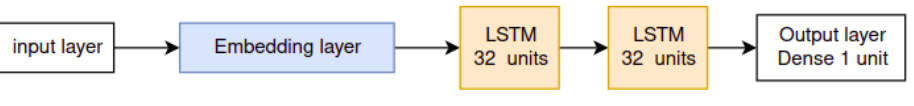
\includegraphics[width=\linewidth]{basemodel.png}
  \caption{Base model structure.}
  \label{fig:basemodel}
\end{figure}

\subsection{Metrics}
The evaluation method for this binary classification task is the micro-averaged F1 score between predicted and expected answers. F1 is calculated as follows: 
\begin{equation}
  F1 = 2\times \frac{precision\times recall}{precision+recall},
\end{equation}
where 
\begin{equation}
  precision = \frac{TP}{TP+FP},
\end{equation}
\begin{equation}
  recall = \frac{TP}{TP+FN}.
\end{equation}
TP, FP, and FN stands for true positive, false positive, and false negative; respectively.

Given the nature of the task is disaster classification, we are more interested in having a perfect Recall which means that out of all positive records (real disaster) how many records are predicted correctly because missing a real disaster is more unfortunate than predicting a fake disaster. The advantage of choosing the Recall as an alternative metric is that we are less likely to miss a real disaster. However, the disadvantage of this metric over F1 score is that we will have worse precision. 

\section{Results}
\subsection{Training setting}
The implementation has been done by Tensorflow, and Keras libraries \cite{keras}. We used Colab-pro's GPU for the training process. The train and test datasets have 7613 and 3263 data samples, respectively; 20\% of train data randomly selected to be the validation dataset. The low amount of data allows us to perform K-fold cross-validation (K=2, in our case) over the training process, and three epochs for each fold with the batch size equals to 32. The activation function for dense layer and output layer is set to \textit{tanh} and \textit{sigmoid} respectively. The \textit{binary crossentropy} is chosen as the loss function. The parameters correspond to BERT transformer is set to be trainable during training process.  

\subsection{Hyper-parameter optimization}
As specified by the original paper of the BERT \cite{devlin2018bert}, the optimizer used is Adam, with a leaning rate between 2e-5 and 5e-5. Since the BERT layer plays a key role in our model, the optimization of learning rate will be selecting the learning rate between 2e-4, 2e-5, 2e-6. In Tab. \ref{tab:lexp}, the results for different learning is shown. The 2e-5 gives the best F1-score performance and we proceed the training process with this value.

\begin{table}
  \caption{Adam's learning rate optimization experiment}
  \label{tab:lexp}
  \begin{tabular}{ccl}
    \toprule
    Learning rate&F1-score\\
    \midrule
    2e-4 & 0.57\\ 
    \textbf{2e-5} & \textbf{0.83}\\ 
    2e-6 & 0.80\\ 
  \bottomrule
\end{tabular}
\end{table}

As a second hyper-parameter in different experiments we try to find best regularization schemes for our problem, L1, L2, and L1\&L2 are used for the hidden dense layer. L2-norm has slightly better performance as you can see in Tab. \ref{tab:rexp}
\begin{table}
  \caption{Regularization scheme optimization experiment}
  \label{tab:rexp}
  \begin{tabular}{ccl}
    \toprule
    Regularization scheme&F1-score\\
    \midrule
    L1 &0.8176\\ 
    L2(0.001)  &0.8235\\ 
    \textbf{L2(0.01)}  &\textbf{0.8302}\\ 
    L2(0.1)  &0.8219\\ 
    L1\&L2(0.01) &0.8234\\
  \bottomrule
\end{tabular}
\end{table}

\subsection{Final results}
In the Kaggle competition correspond to this task, the micro average F1-score was considered as metric. F1-score comparison between the trained proposed model and base model for test dataset is shown In Tab. \ref{tab:result}. Proposed model beats the base model on the same train, test, validation splitting dataset. 

Finally, we provide a very good example to illustrate the strength of the proposed model. In Fig. \ref{fig:pred} you can see how the proposed model can understand the context of the tweet where the base model failed to predict correctly and probably was deceived by the negative words inside the text (e.g. hate, bleeding, scratch, bite).  


\begin{figure}[h]
  \centering
  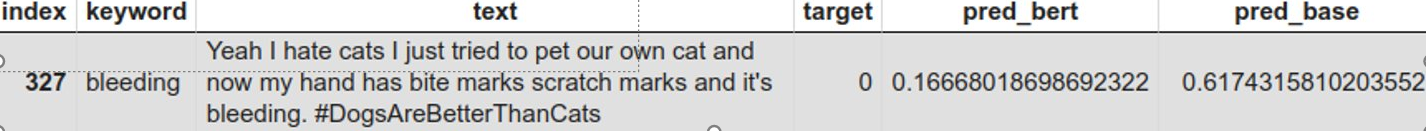
\includegraphics[width=\linewidth]{pred.png}
  \caption{Prediction example.}
  \label{fig:pred}
\end{figure}



\begin{table}
  \caption{Regularization scheme optimization experiment}
  \label{tab:result}
  \begin{tabular}{ccl}
    \toprule
    Model&F1-score\\
    \midrule
    Base model (LSTM) &0.78\\ 
    Proposed model (BERT)  &\textbf{0.83}\\ 
  \bottomrule
\end{tabular}
\end{table}

\section{Discussion}

One big limitation with the dataset is that in some tweets there is not much information to tell. For example, e.g. "CHECK THIS PICTURE OUT!!!"; this tweet can be interpreted as a disaster or not a real disaster because it refers to a picture that is not provided in the dataset. From our standpoint of view, the dataset can significantly be improved by at least providing features like pictures, number of retweets, and number of likes or dislikes.

There is also an ethical issue with this dataset. Since the dataset contains text that may be used slang words, there is no clear solution to find out how are they distributed in the dataset. For example, if we assume in this specific dataset that slang words are most used for real disaster tweets, then the trained model will be slang biased and will predict the tweets that include the slang words as a real disaster tweet.


\section{Conclusions}
The disaster tweet classification was the task that we engaged in with this project. During dataset analysis, we illustrated that \textit{keyword} feature has some correlation with the target and can be used along the \textit{text} feature. Then, we came up with the structure that uses both features in the BERT transformer. For the sake of comparison, we also provide a base model with an LSTM structure based on what we discussed in the related work section. The proposed model structure outperforms the competitive base model by a about five percent improvement in terms of F1 score. 





%%
%% The next two lines define the bibliography style to be used, and
%% the bibliography file.
\bibliographystyle{ACM-Reference-Format}
\bibliography{sample-base}


\end{document}
\endinput
%%
%% End of file `sample-sigconf.tex'.
